\ifx\allfiles\undefined

	% 如果有这一部分另外的package,在这里加上
	% 没有的话不需要
	
	\begin{document}
\else
\fi
    \chapter{整数规划}
    \section{整数规划问题与数学模型}
    \subsection{整数规划问题的定义}
    在前面的线性规划和运输规划问题中,最优解一般都是实数。但对于实际中的具体问题的解常常要求必须取整数,即称为整数解,
例如,问题答案是几个人、几台设备、几辆车等,无法用实数表达。因此,对于要求最优整数解的问题,就涉及到整数规划。
\begin{dfnbox}{整数规划}{amznotes}
    如果一个数学规划的\textcolor{red}{某些决策变量或全部决策变量}要求必须取\textcolor{red}{整数},则这样的问题称为\textbf{整数规划问题};
相应的模型称为\textbf{整数规划模型}、
\end{dfnbox}
\begin{itemize}
    \item \textbf{纯整数规划问题}:所有的决策变量都为\textcolor{red}{非负整数}的整数规划;
    \item \textbf{混合整数规划问题}:存在决策变量为\textcolor{red}{负整数}的整数规划;
    \item \textbf{0-1规划}:所有的决策变量只能取\textcolor{red}{0或1}的整数规划;
\end{itemize}

\subsection{整数规划问题的数学模型}

\begin{thmbox}{一般形式的整数线性规划问题}{cool}
    \[
    \max(\min) \ z = \sum_{j=1}^{n} c_j x_j
    \]
    s.t.
    \[
    \begin{cases}
        \sum_{j=1}^{n} a_{ij} x_j \leq (\geq, =) b_i \,, & (i=1,2,\dots,m) \,, \\
        x_j \geq 0 \,, \quad x_j \text{ 为整数} & (j=1,2,\dots,n) \,.
    \end{cases}
    \]
\end{thmbox}

\begin{exbox}{\textbf{产品生产(纯整数规划问题)}}
    1\textbf{例}:某厂生产 $A_1$ 和 $A_2$ 两种产品,需要经过 $B_1$、$B_2$、$B_3$ 三道工序加工。单件工时和利润值以及各工序每月工时定额表 2-1。问工厂应如何安排生产才能使总利润最大?
    
    \begin{table}[H]
        \centering
        \label{tab:2-1}
        \renewcommand{\arraystretch}{1.5}
        \begin{tabular}{|c|c|c|c|c|}
            \hline
            & $B_1$ & $B_2$ & $B_3$ & 利润(元/件) \\ \hline
            $A_1$ & 0.3 & 0.2 & 0.3 & 25 \\ \hline
            $A_2$ & 0.7 & 0.1 & 0.5 & 40 \\ \hline
            工时定额(小时/月) & 250 & 100 & 150 & \\ \hline
        \end{tabular}
        \caption{工厂加工条件与利润}
    \end{table}
    
    \textbf{解:} 根据表 4-1 的最后一栏的利润数据,生产 $A_1$ 件、$A_2$ 件能获取的总利润为 $25x_1 + 40x_2$,因此,该问题的数学模型为:
    \begin{equation}
        \max \quad 25x_1 + 40x_2 \label{eq:Chapter4_obj_1}
    \end{equation}
    约束条件:
    \begin{align}
        0.3x_1 + 0.7x_2 &\leq 250 \,, \label{eq:c1} \\
        0.2x_1 + 0.1x_2 &\leq 100 \,, \label{eq:c2} \\
        0.2x_1 + 0.5x_2 &\leq 150 \,, \label{eq:c3} \\
        x_1 \geq 0 \,, \quad x_2 &\geq 0 \,. \label{eq:Chapter4_nonneg_1}
    \end{align}
    这是一个纯整数规划问题。
    
    \textbf{解}:设工厂每月生产 $A_1$ 产品 $x_1$ 件,$A_2$ 产品 $x_2$ 件。则按表 2-1 提供的条件数据,$A_1$ 产品 $x_1$ 件、$A_2$ 产品 $x_2$ 件加工需要的总利润为 $25x_1 + 40x_2$,因此,该问题的数学模型为:
    \begin{equation}
        \max \quad 25x_1 + 40x_2
    \end{equation}
    约束条件:
    \begin{align}
        0.3x_1 + 0.7x_2 &\leq 250 \,, \tag{$B_1$ 工序,工时限制} \\
        0.2x_1 + 0.1x_2 &\leq 100 \,, \tag{$B_2$ 工序,工时限制} \\
        0.2x_1 + 0.5x_2 &\leq 150 \,, \tag{$B_3$ 工序,工时限制} \\
        x_1 \geq 0 \,, \quad x_2 &\geq 0 \,. \tag{且只能整数}
    \end{align}
    另外,由于 $x_1$ 为 $A_1$ 的件数,因此 $x_1 \geq 0$ 且只能取整数;同理,$x_2 \geq 0$ 且只能取整数。
\end{exbox}


\begin{exbox}{\textbf{背包问题(0-1规划)}}
    1\textbf{例}:一个背包的总容积为 $V$,现要在 $n$ 种物品中选择。设物品 $j$ 的重量为 $w_j$,体积为 $v_j$,$j=1,2,\dots,n$。问如何选择,使得到的总价值最大,且总重量不超过 $V$,又使装的总重量最大。这一个题目有 $n$ 个约束情况,如装某类装箱,装箱,装车等。
    
    \textbf{解:} 设对于物品 $j$,变量
    \[
    x_j = \begin{cases} 
        1 & \text{物品 $j$ 被装入背包} \\ 
        0 & \text{物品 $j$ 不被装入背包}
    \end{cases} \quad j=1,2,\dots,n
    \]
    则所有被选择装物品的总体积为 $\sum_{j=1}^{n} v_j x_j$,总重量为 $\sum_{j=1}^{n} w_j x_j$,该问题的数学模型为:
    \begin{equation}
        \max \sum_{j=1}^{n} w_j x_j \label{eq:Chapter4_obj_2}
    \end{equation}
    约束条件:
    \begin{align}
        \sum_{j=1}^{n}  &v_j x_j\leq V \,, \label{eq:constraint} \\
        x_j &= 0, 1 \,, \quad j=1,2,\dots,n \,. \label{eq:binary}
    \end{align}
    这是一个 0-1 规划问题。
\end{exbox}


    \section{一般整数规划的求解方法—分支定界法}
    为了解决整数规划问题,我们自然想到两种办法:
    \begin{itemize}
        \item 想到第二章提到的下料问题,可以用线性规划求解,结果四舍五入;
        \item 反正是整数,不妨穷举求解;
    \end{itemize}
    显然第一个方法不够靠谱,第二个方法效率太低。\\
    \begin{exbox}{\textbf{第一个方法不靠谱的原因}}
    1例如, 考虑如下整数规划问题:
    \begin{align}
        \max \ 3x_{1} &+ 13x_{2} \\
        \text{s.t.} \quad 2x_{1} + 9x_{2} &\leq 40 \\
        11x_{1} - 8x_{2} &\leq 82 \\
        x_{1} \geq 0, \quad x_{2} &\geq 0 \quad \text{且取整数}
    \end{align}
    画出可行域如下所示\footnote{图中可以看到,浮点数最优解 B四周的四个整数点都不在可行域内,四舍五入的结果是错误的。反而整数最优解在C点。}:
    \begin{figure}[H]
        \centering
        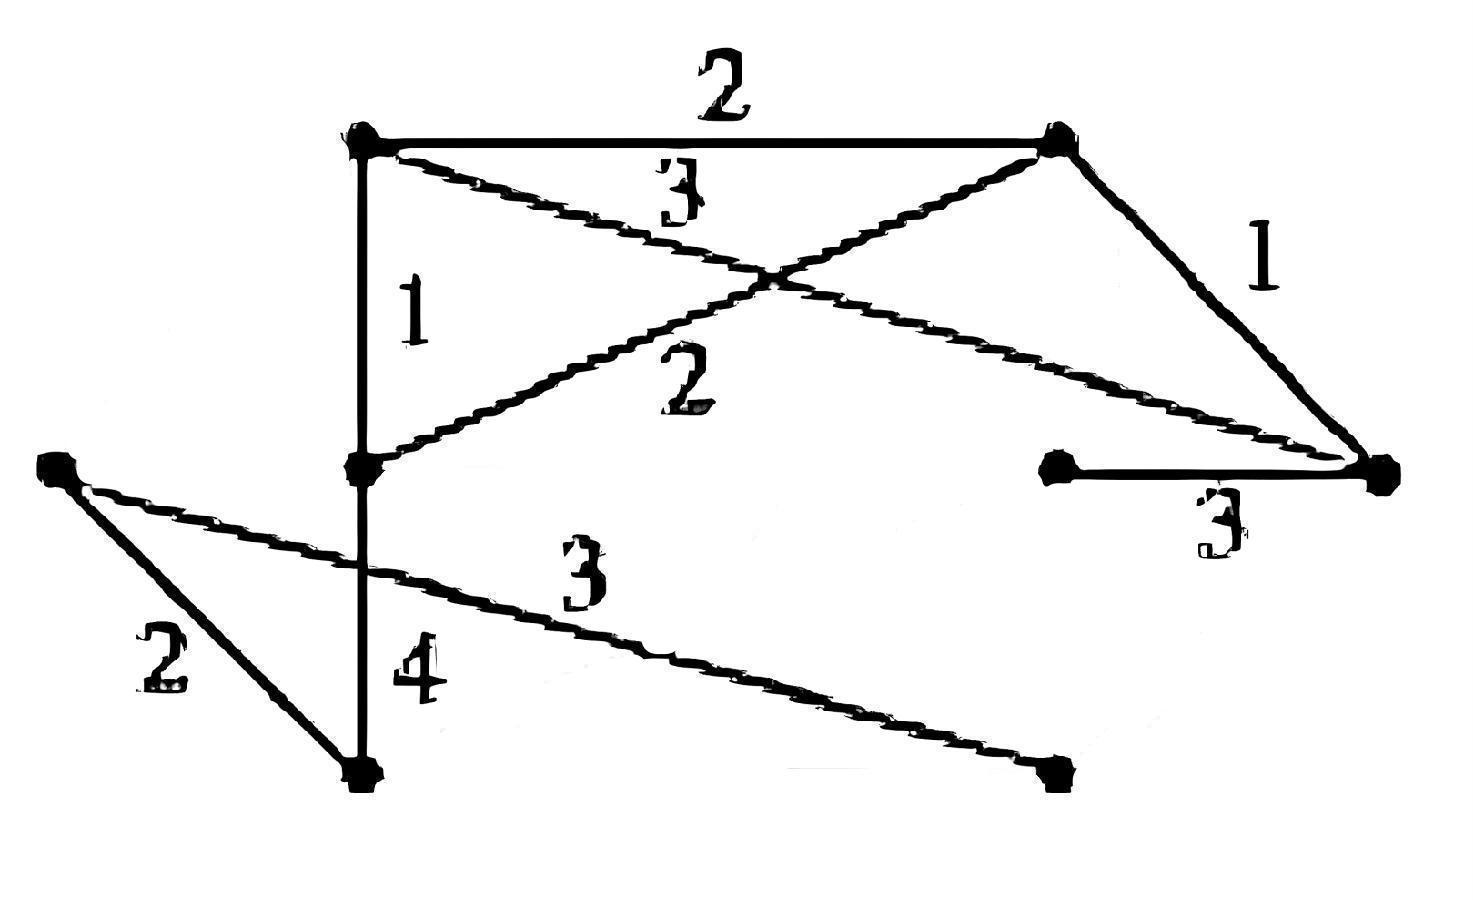
\includegraphics[width=0.8\textwidth]{8.png}
        \caption{整数规划的四舍五入求解}
        \label{fig:Chapter4_Temporary_Pavilion_1}
    \end{figure}
    \end{exbox}

    目前,常用的求解整数规划的方法是分枝定界法和割平面法。作为一种最基本的方法,下面介绍分枝定界法。
    \begin{notebox}{\textbf{分枝定界法}}
        \\
        \begin{enumerate}
            \item 设有最大化的整数规划问题A,与它相应的线性规划问题(即在整数规划中去掉了决策变量的整数取值要求)为B,设二者的最优值分别为$z_A^*$和$z_B^*$;
            \item 从解问题B开始,若B的最优解符合A中的整数条件,\textcolor{red}{则A的最优解即为B的最优解},结束;
            \item 若B的最优解不符合A的整数条件,则B的最优解对应的最优值$z_B^*$一定是\textcolor{red}{A的最优值$z_A^*$的上界},记为$\overline{z}$ ,而A的某一\textcolor{red}{任一可行解}(即任意一个整数解)的目标函数值将是一个下界$\underline{z}$。此时$\underline{z}\leq z_A^* \leq \overline{z}$,称为\textbf{定界};
            \item 分枝定界法即不断将B的可行域分成子区域(称为\textbf{分枝}),并在每个子区域中确定A的\textcolor{red}{上界$\overline{z}$和下界$\underline{z}$}的方法,逐步夹逼,直到找到A的最优解为止;
        \end{enumerate}
    \end{notebox}

    \begin{figure}[H]
        \centering
        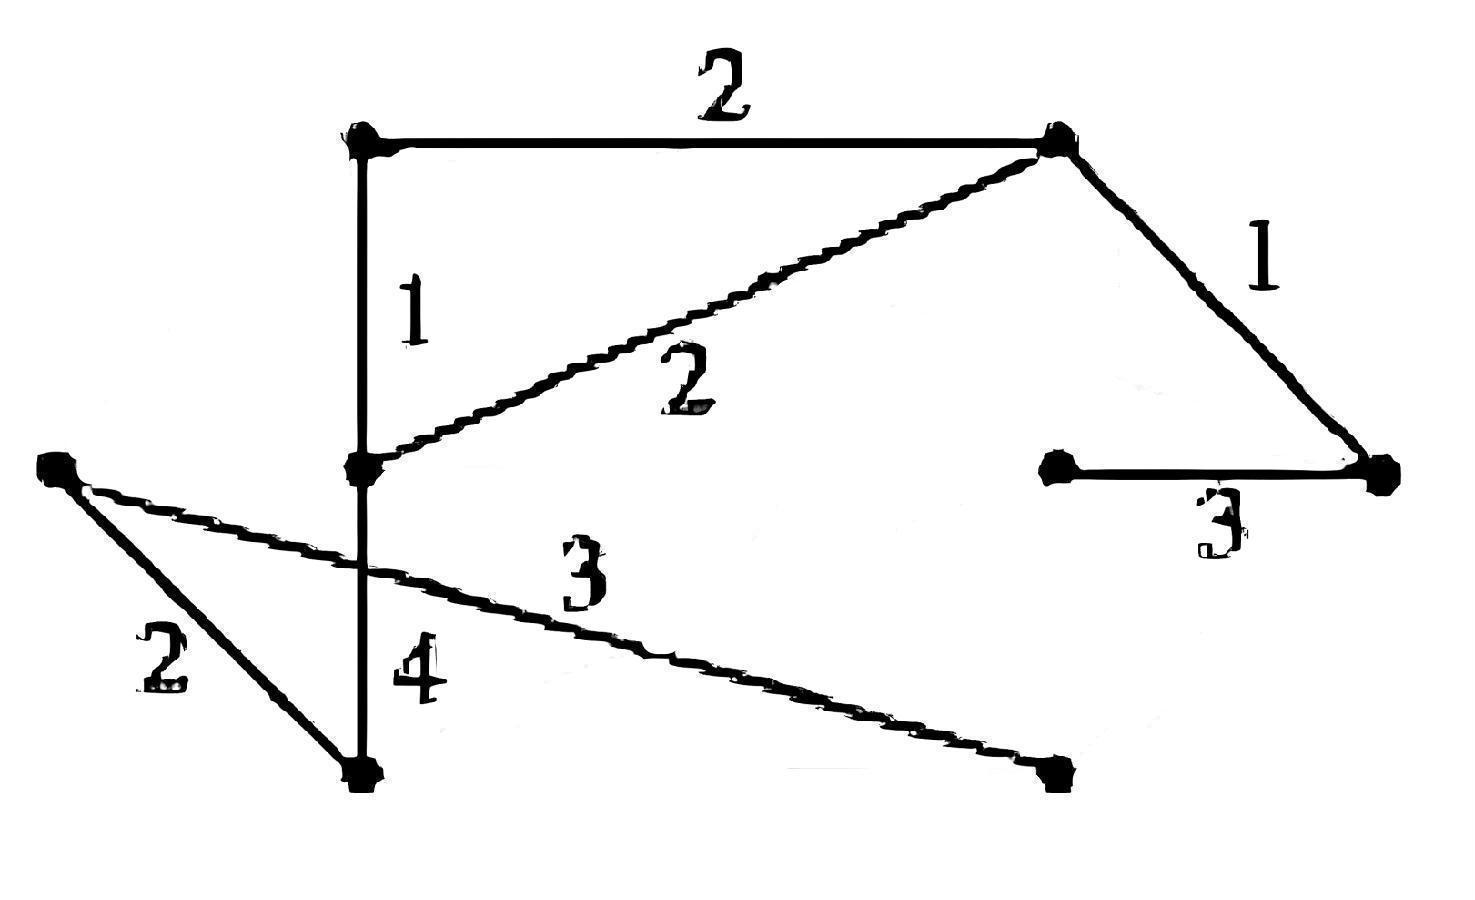
\includegraphics[width=0.5\textwidth]{9.png}
        \caption{分枝定界法过程}
        \label{fig:Chapter4_Temporary_Pavilion_2}
    \end{figure}
    \begin{exbox}{\textbf{分枝定界法}}
        1\textbf{例:}\ 考虑如下整数规划问题:
        \begin{align}
            \max \ 40x_{1} &+ 90x_{2} \\
            \text{s.t.} \quad 9x_{1} + 7x_{2} &\leq 56 \\
            7x_{1} + 20x_{2} &\leq 70 \\
            x_{1} \geq 0, \quad x_{2} &\geq 0 \quad \text{且取整数}
        \end{align}
        \textbf{解:}\ 记上述原问题为A。先考虑A中去掉整数约束条件后的线性规划问题B.
        \begin{figure}[H]
            \centering
            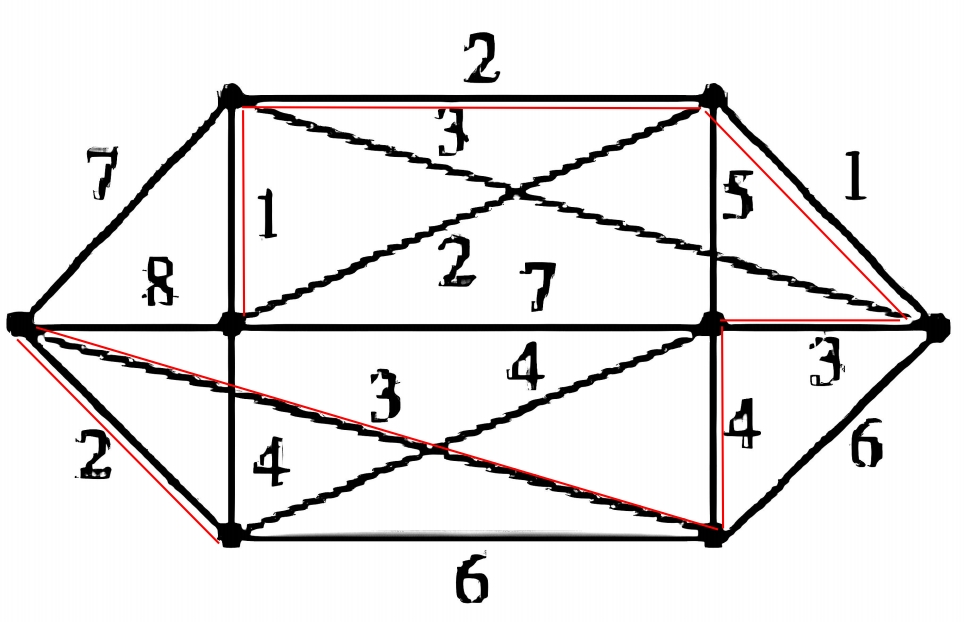
\includegraphics[width=0.8\textwidth]{11.png}
            \caption{问题B的图解分析}
            \label{fig:Chapter4_Temporary_Pavilion_3}
        \end{figure}
        \begin{figure}[H]
            \centering
            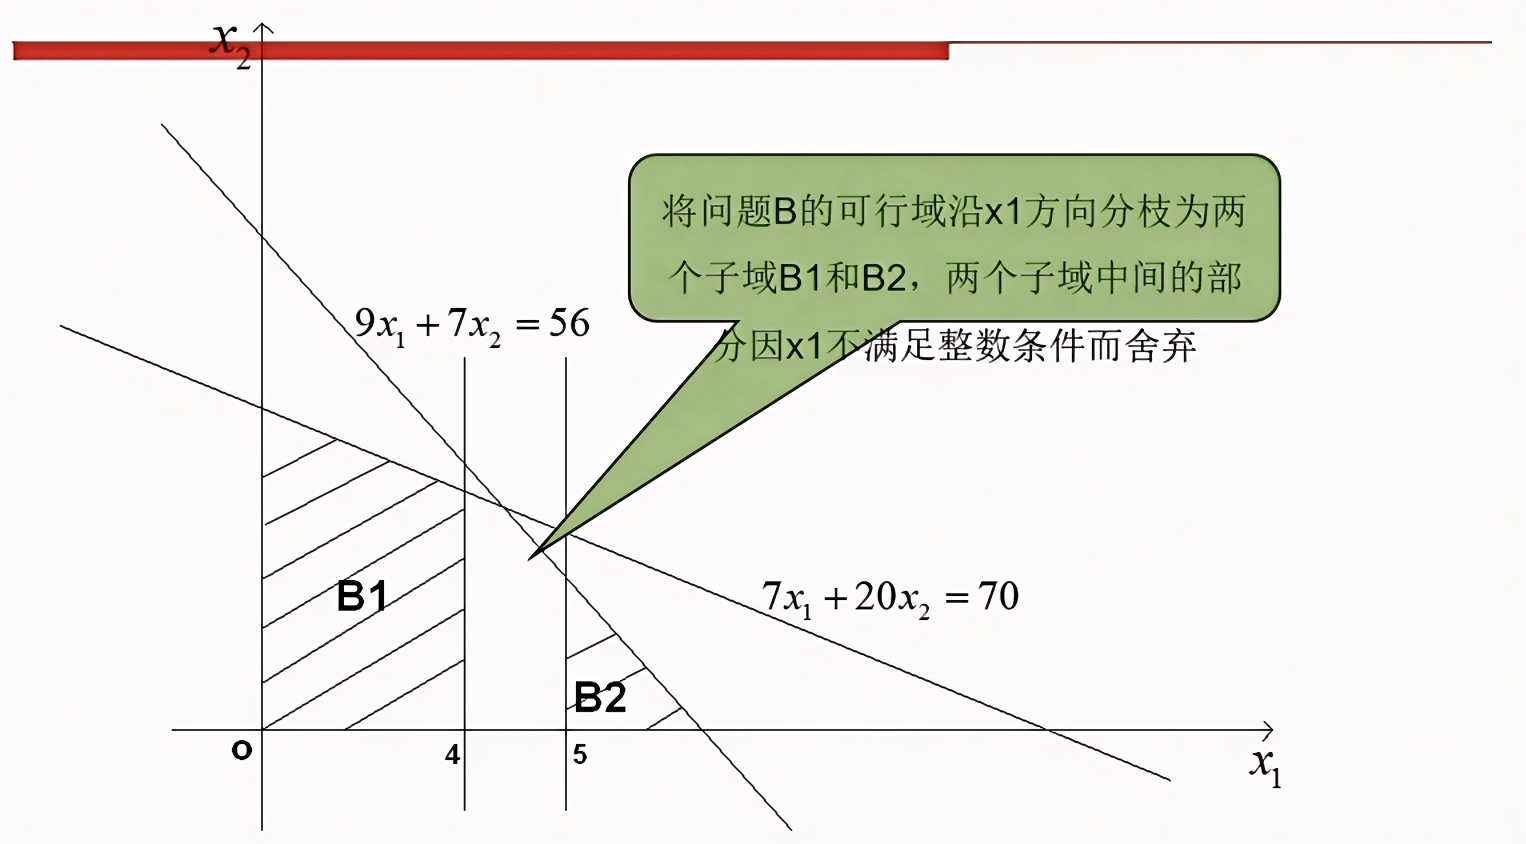
\includegraphics[width=0.8\textwidth]{10.png}
            \caption{问题B的分枝}
            \label{fig:Chapter4_Temporary_Pavilion_4}
        \end{figure}
        \end{exbox}
    


    \section{0-1规划及其求解方法}
    \section{案例分析}
    

\ifx\allfiles\undefined
	
	% 如果有这一部分的参考文献的话,在这里加上
	% 没有的话不需要
	% 因此各个部分的参考文献可以分开放置
	% 也可以统一放在主文件末尾。
	
	%  bibfile.bib是放置参考文献的文件,可以用zotero导出。
	% \bibliography{bibfile}
	
	end{document}
	\else
	\fi